\begin{figure}[htbp]
	\centering
	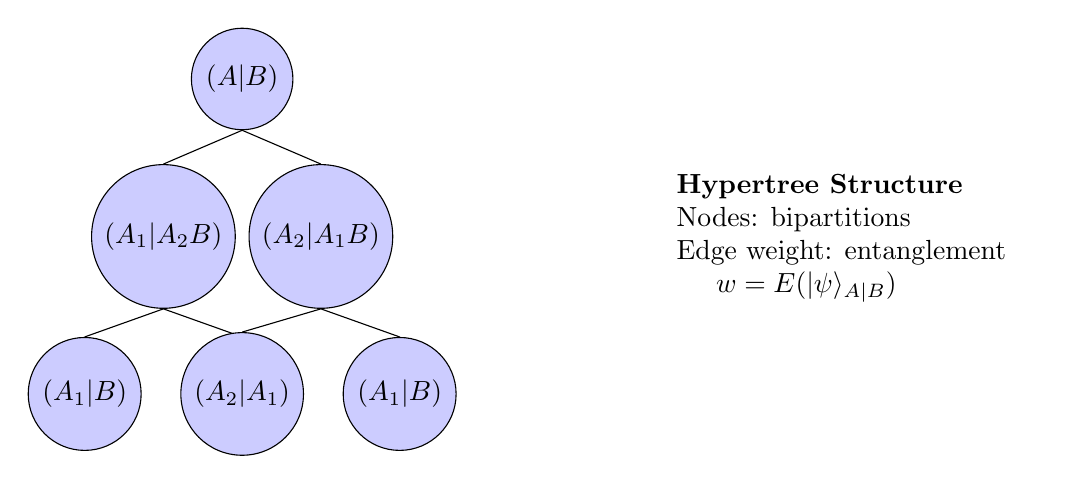
\begin{tikzpicture}[
			level distance=2cm,
			sibling distance=2cm,
			edge from parent path={(\tikzparentnode.south) -- (\tikzchildnode.north)},
			every node/.style={draw, circle, fill=blue!20, minimum size=1cm}
		]
		\node {$(A|B)$}
		child {
				node {$(A_1|A_2B)$}
				child {
						node {$(A_1|B)$}
					}
				child {
						node {$(A_2|B)$}
					}
			}
		child {
				node {$(A_2|A_1B)$}
				child {
						node {$(A_2|A_1)$}
					}
				child {
						node {$(A_1|B)$}
					}
			};

		\node[draw=none, fill=none, right=1cm] at (4,-2) {
			\begin{tabular}{l}
				\textbf{Hypertree Structure} \\
				Nodes: bipartitions          \\
				Edge weight: entanglement    \\
				\hspace{0.5cm}$w = E(|\psi\rangle_{A|B})$
			\end{tabular}
		};
	\end{tikzpicture}
	\caption{Hypertree representation of multipartite entanglement. Each node represents a bipartition of the system, and edge weights quantify the entanglement across that cut. This hierarchical structure reveals the nesting of entanglement in tensor network states.}
	\label{fig:hypertree}
\end{figure}
